\part{Seminar 11 - Modern Electrical Machine Design Optimization:
Techniques, Trends, and Best Practices}

\makebox[.33\textwidth]{Nicolas Colsoul}\makebox[.33\textwidth]{Frédéric Jadoul}\makebox[.33\textwidth]{Michaël Oudraogo}

\section{Introduction}
L'optimisation est une notion très large qui peut s'appliquer à tous les domaine. Pour ce qui concerne les machine électriques
\begin{itemize}
    \item elles sont très utilisées dans diverses applications (dans l'industrie, pour la production d'énergie)
    \item elle sont de plusieurs types (moteur, générateur, synchrone, asynchrone, etc)
    \item de taille différentes (de l'ordre du centimètre au dizaine de mètres)
    \item de puissance différente (milliwatt-megawatt)
\end{itemize}
Au vu de cette variété, il est important d'optimiser les machines électrique pour répondre à une utilisation dans des conditions bien précises (slides 2 à 5).
\section{Problème d'optimisation}
Un problème d'optimisation comporte principalement 4 étapes de façon générale : 
\begin{enumerate}
    \item La définition des objectifs et des contraintes
    \item La définition de l'espace de recherche
    \item L'exploration de l'espace de recherche et l'obtention de l'espace de solution
    \item L'évaluation et l'interprétation des résultats.
\end{enumerate}

Partant du problème jusqu'à la solution, l'optimisation est un problème récursif et non séquentiel. Les deux première étapes étant plus configurées par l'ingénieur tandis que les deux dernières forment la boucle itérative (slides 7 et 8).
\begin{figure}[H]
    \centering
    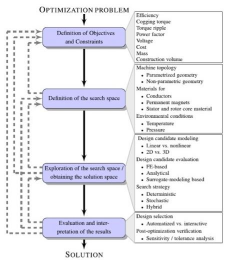
\includegraphics{Process.png}
    \caption{Processus d'optimisation}
    \label{fig:Optimisation}
\end{figure}
\section{Objectifs et contraintes}
Pour obtenir de bonne solutions il est important de définir le problème. Les objectif à maximiser ou minimiser et les conditions (contraintes) de résolution du problème. On peut distinguer les problèmes à objectif unique "single objective" et à objectif multiple "multiple objective". 
\begin{figure}[H]
    \centering
    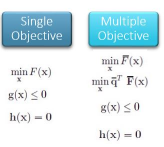
\includegraphics{Objectif.png}
    \caption{Fonctions objectifs}
    \label{fig:objection}
\end{figure}
De la figure \ref{fig:objection}, nous pouvons voir la définition de la fonction objectif $F$ à minimiser et des contraintes $G$ (inégalité) et $H$ (égalité) à respecter. Dans le cas du du multiple objectif $F$ est plutôt un vecteur qui peut s'accompagner d'un vecteur poids $q$. Un problème à objectif multiple pure et dur serait d'avoir des poids égaux, dans ce cas il est possible d'utiliser des méthodes d'évaluation de problèmes à objectif unique pour évaluer des problèmes à objectif multiples : le produit scalaire entre le vecteur poids $q$ et le vecteur objectif donne bien un scalaire. 
\begin{figure}[H]
    \centering
    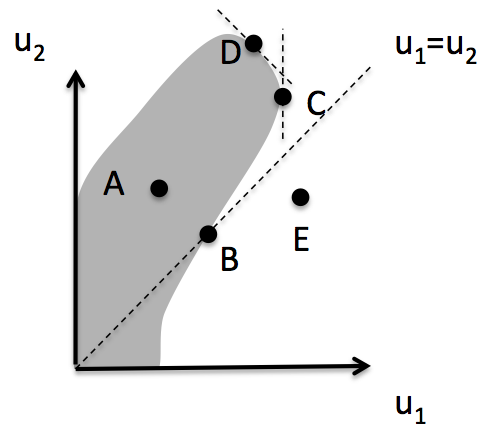
\includegraphics{pareto.png}
    \caption{Front de pareto optimum}
    \label{fig:Pareto}
\end{figure}
Le front de Pareto illustré par la figure \ref{fig:Pareto}, nous rappel que la solution d'une optimisation est généralement un compromis entre différents objectifs. Dans le cas de deux objectifs à maximiser, quand on maximise A, on diminue B et vice versa.

\section{Définition de l'espace de recherche}
Dans un premier temps il faut faire la différence entre le changement de topologie et le changement de forme. Par exemple un donut et une tasse ont la même topologie, un trou entouré de matière (slide 12). 

La définition de la géométrie est la principale étape qui définit la base des solutions possibles. Elle peut être paramétrée ou non paramétrée. Dans le cas paramétrée, le paramètre peut être continue (une longueur, par exemple) ou discontinue (un nombre de paire de pôle, par exemple). Le choix des paramètres doit être fait de façon judicieuse à réduire le nombre d'évaluations. Par exemple, la définition d'une géométrie cylindrique peut être faite en choisissant comme paramètre le rayon intérieur et le rayon extérieure $ R_i$ et $R_e$; cependant une solution avec $R_i>R_e$ n'a pas de sens, il est plus intelligent de définir un paramètre $\alpha$ tel que $R_i = \alpha \cdot R_e$  avec $\alpha$ compris entre 0 et 1.  Les géométries paramétrées fixent la forme de la solution limitant ainsi le nombre de résultats tandis que les géométries non-paramétrées génèrent plus de possibilités de solutions parfois exotiques. 

Après l'exemple du cylindre qui est une optimisation de forme, il y a l'exemple d'une optimisation de topologie d'une machine synchrone à reluctance qui a été optimisée par la méthode d'optimisation binaire. La surface du rotor est maillé, puis chaque maille est rempli soit par de l'air ou de l'acier (slides 13 et 14). Enfin, en faisant attention au choix du paramètre, en privilégiant une structure symétrique ou en choisissant la bonne technique d'évaluation (discrète ou analytique) on peut réduire la complexité et le temps  des calculs (slide 15).

\section{Exploration de l'espace de solution}
\subsection{Plans d'exercice (Design Of Experiments)}
L'idée est de réduire le nombre d’expérience à faire pour prendre une décision sur une fonction objectif et gagner du temps et de l’argent. Tester quelques valeurs des paramètres d’entrée pour voir leur influence sur le problème et les interactions entre eux. 

\paragraph{Approche mathématique :} trouver une relation linéaire ou quadratique entre les facteurs d’entrée.
$2N + C(N,2)$ constantes à définir et donc points à évaluer dans l’espace de solution mais on ne sait pas forcément lesquels choisir.

\paragraph{Approche factorielle :} trouver une relation linéaire seulement en ne prenant que la valeur normalisée la moins élevée $(-1)$ et la plus élevée $(1)$.
Ce qui donne $2^k$ expériences à faire. Problème rencontré : parfois le nombre d’expérience est encore trop important, ne donne parfois pas assez d’informations car on ne regarde pas ce qu’il se passe pour les valeurs intermédiaires.

\paragraph{Plan d’expérience optimisé :} Box-Behnken design, Latin hypercube, matrice d’Hadamard, plan centré composite, ...

Box-Behnken Design : exemple avec 3 paramètres ($x_1$ , $x_2$ et $x_3$) et trois niveau pour chaque paramètre ($-1$, $0$, $1$). 27 possibilités mais il suffit d’évaluer la fonction objectif pour les points bleu (13 expériences au total).

\begin{figure}[H]
    \centering
    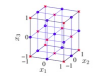
\includegraphics{Box-Behnken.png}
    \caption{Box-Behnken Design}
\end{figure}
\subsection{Techniques d'évaluation et modèle suppléant "surrogate"}
\subsubsection*{Techniques d'évaluation}
les fonctions objectifs ou de contrainte peuvent être discrètes ou analytiques. 
\begin{itemize}

    \item \textbf{fonction analytique}\\
    Elle peut être rapidement implémenter pour l'évaluation rapide d'un grand nombre de machine différente. Elle est généralement lié à une topologie de machine et est amélioré grâce au résultats des expériences. Elle permet l'obtention de résultats précis mais n'arrive pas à fournir des information sur les effets locaux.
    \item \textbf{fonction discrète} \\
    Elle permet une investigation plus détaillée de la machine et aussi d'analyser plusieurs objectifs simultanément.Elle est surtout limité par la puissance de calcule des ordinateurs.De nos jours des simulation 3-D sont même possible à cause de l'explosion de la puissance des ordinateurs (silde 24).
\end{itemize}
\subsubsection*{ modèle suppléant "surrogate"}
C'est un modèle sensé modélisé le comportement de la machine. Elle permet de représenter une machine très complexe, sur laquelle on ne possède que quelques informations. Cette représentation est faite à partir d'un échantillon de points qui serviront à la construction du modèle. Des fonctions polynomiales sont utilisées pour décrire le fonctionnement de la machine.Dans le cas par exemple où l'évaluation des performances d'une machine sont longue et/ou coûteuse,un modèle surrogate construit à partir de quelques évaluations permet une économie de temps et d'agent. Cependant ça reste une approximation et basé sur des échantillons qui peuvent contenir des erreurs. \\ Quelques exemples de modèle surrogate sont:RSM (Response surface methodology)
Artificial neural networks; Kriging; Support vectors machine; RBF (Radial basis functions)
\subsection{Optimisation de la fonction objectif}
\subsubsection{Optimisation déterministe}
\begin{itemize}
    \item Utilisée pour trouver une valeur avant le processus d’évaluation 
    \item Toujours les mêmes résultats avec le même problème et les même conditions initiales
    \item Peut rester coincée dans les extrema locaux (exemple : si on commence à un point de l’espace de solution proche d’un extrema local, on restera toujours coincé à cet extrema si on refait l’expérience)
    \item Peut prendre trop de temps si nous devons explorer tout l’espace de solution
\end{itemize}

Exemple : méthode du gradient (maximum d’une fonction avec la dérivée), grid search, Newton, ...

\paragraph{Méthode de Newton :} méthode plus directe que la méthode du gradient (prend en compte la dérivée seconde)

\begin{figure}[h!]
    \centering
    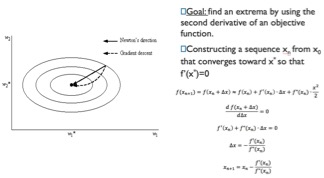
\includegraphics{Newton_method.png}
    \caption{Méthode de Newton}
\end{figure}

\subsubsection{Optimisation stochastique}
\begin{itemize}
    \item Principe : utiliser des variables aléatoires comme variables d’entrée pour explorer l’espace de recherche des solutions.
    \item Ne reste pas bloqué dans les extrema locaux
    \item La fonction objectif ne doit pas être dérivable
    \item Ne donne pas forcément la solution exacte
\end{itemize}
Exemple : PSO (Particle warm Optimization), DE (differential evolution), NSGA-2 (Non-dominated sorting genetic algorithm), ...

\paragraph{PSO (Particle Swarm Optimisation) :} prendre en compte les interactions entre les individus pour trouver le plus rapidement une solution (comme le font les oiseaux,  les colonies d’abeilles, etc).

4 paramètres :

\begin{itemize}
    \item $x_i$ la position actuelle
    \item $v_i$ la vitesse actuelle
    \item $x_{i,best}$ la meilleure position de la particule x jusqu’à présent
    \item $x_{g,best}$ la meilleure position du groupe de particules 
\end{itemize}

2 équations par récurrence :

\begin{itemize}
    \item $x_i(t)=x_i(t-1)+v_i(t)$
    \item $v_i(t+1)= \omega v_i(t) +c_1r_1[x_{best,i}(t)-x_i(t)]+c_2r_2[x_{gbest,i}(t)-x_i(t)]$
\end{itemize}

Avec $\omega$ l’inertie, $c_1$ et $c_2$, 2 constantes à déterminer et $r_1$ et $r_2$, 2 nombres aléatoires compris entre 0 et 1.

\begin{figure}[H]
    \centering
    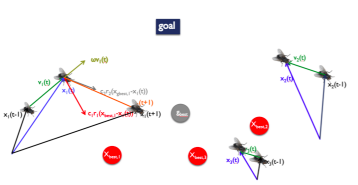
\includegraphics[width=120mm]{PSO-1.png}
    \caption{Exemple avec des mouches}
\end{figure}

\begin{figure}[H]
    \centering
    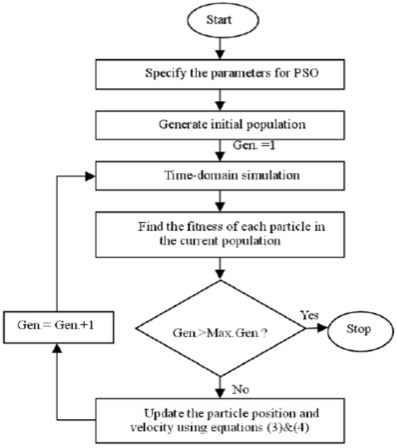
\includegraphics[width=100mm]{PSO-2.png}
    \caption{PSO flowchart}
\end{figure}

\paragraph{NSGA-2 (Non-dominated sorting genetic algorithm) :} algorithme d’évolution basé sur la génétique multi-objectif.

Principe : garder pour chaque génération les meilleures individus tout en gardant une diversité (grâce à la crowding distance), retourne un ensemble de point qui est la solution au sens Pareto optimal du problème.

\begin{figure}[H]
    \centering
    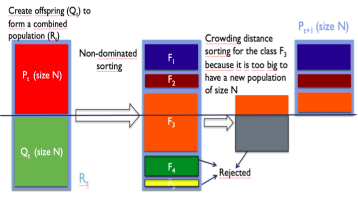
\includegraphics[width=100mm]{NSGA-1.png}
    \caption{Principe général pour une itération}
\end{figure}

\begin{figure}[H]
    \centering
    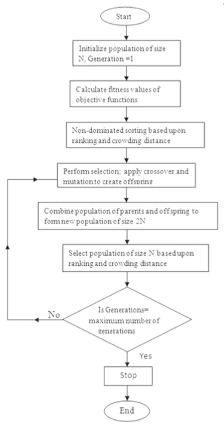
\includegraphics[width=60mm]{NSGA-2.png}
    \caption{NSGA-2 flowchart}
\end{figure}


\url{ https://www.youtube.com/watch?v=SL-u_7hIqjA&list=WL&index=2&t=0s}


\section{Exemple}
Un autre papier (également disponible sur Moodle) présente l'optimisation d'une machine convertisseur de vagues. Bien que le contenu de ce papier est suffisant pour en faire un séminaire complet (années précédentes), c'est également un très bon exemple pour illustrer la méthodologie précédemment expliquée.

\subsection{Présentation du problème}
On veut optimiser un convertisseur de vague. C'est une machine qui utilise l'énergie des vagues pour produire de l'électricité. Elle est composée de deux parties principales : une machine à aimant permanent monté en surface (SPM) et d'un convertisseur de puissance AC - DC - AC basé sur des IGBT.

On rencontre déjà 2 difficultés :
\begin{itemize}
    \item La vitesse du rotor est variable : forcément, elle dépend des vagues. On veut que la machine soit optimisée tout le temps (i.e pour n'importe quelle vitesse). On nous donne une caractéristique connue couple-vitesse pour laquelle toute la machine doit être optimisée.
    
    $\rightarrow$ Optimisée pour tout $(T_i;\Omega_i)$ où $i$ désigne un point de la caractéristique.
    
    \item Il ne suffit pas d'optimiser la machine et ensuite le convertisseur mais bien d'optimiser le tout. Les courants qui les traversent sont, en effet, identiques. 
\end{itemize}
On va vite se rendre compte qu'une optimisation basique ne sera pas suffisante dans notre cas.

\subsection{Définition des objectifs et contraintes}
\subsubsection{Objectifs}
Deux objectifs principaux :
\begin{itemize}
    \item Minimiser le coût de la machine :
    $$ Cost = Cost_{converter} + Cost_{machine}$$
    Où $Cost_{converter} = \alpha S^{\gamma}$ avec $S$ la puissance apparente du convertisseur et $\alpha$, $\gamma$ des paramètres donnés par le constructeur des IGBT que les ingénieurs choisissent.
    
    Où $Cost_{machine} = \sum c_x \cdot m_x$ avec $c_x$ le prix au kilo du matériau $x$ et $m_x$ la masse totale du matériau $x$ dans la machine. 
    \item Maximiser l'énergie électrique :
    $$ E_{elec} = \sum (T_i \Omega_i - P_{loss, i}) d_i$$
    Où $P_{loss,i}$ est la somme de toutes les pertes dans la machine et dans le convertisseur et $d_i$ la durée pendant laquelle le rotor est à couple-vitesse ($T_i$;$\Omega_i$). C'est une intégrale discrète.
\end{itemize}

\subsubsection{Contraintes}
Premièrement, les contraintes instantanées ou encore les contraintes électriques. 
\begin{itemize}
    \item Tension nominale : $\sqrt{v_{d,i}^2 + v_{q_i}^2} \le \sqrt{3}V_{rated}$
    \item Courant nominale : $\sqrt{i_{d,i}^2 + i_{q_i}^2} \le \sqrt{3}I_{rated}$
    \item Saturation : $max(B_i) \le B_{sat}$
    \item Démagnétisation : $H_i \ge -H_k$
\end{itemize}
Note : la contrainte en démagnétisation c'est pour éviter de transformer les aimants permanents en vulgaires ferrailles inutiles.

Après transformation de Park et de Concordia, on peut représenter graphiquement toutes ces contraintes dans le repère quadrature/direct :
\begin{figure}[H]
    \centering
    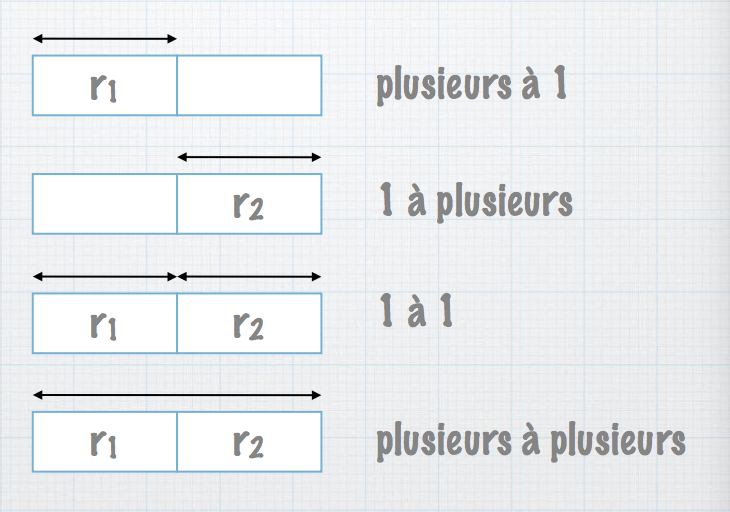
\includegraphics[width=0.5\textwidth]{contraintes.png}
    \caption{Contraintes, représentation graphique}
\end{figure}
On voit tout de suite que le courant de quadrature est fixe (lié au couple) mais que le courant direct va varier et qu'il devra faire partie de l'optimisation. 

Deuxièmement, les contraintes globales ou encore contraintes géométriques.
\begin{itemize}
    \item Contrainte sur l'écart entre le rotor et le stator
    \item Contrainte sur les entrefers par rapport au rayon maximum
    \item Contrainte sur l'épaisseur des aimants
\end{itemize}
(Les équations sont, selon moi, pas pertinentes mais disponibles au slide 62)

\subsubsection{Définition de l'espace de recherche}
Différents jeux de paramètres :
\begin{itemize}
    \item Fixés par les ingénieurs : tension maximum, rayon maximum, champs magnétique maximum etc. 
    \item A optimiser : grandeurs géométriques, nombre de paires de pôles, nombre de tours des bobinages, etc. 
\end{itemize}
On a définit une plage possible pour chaque paramètres. C'est une géométrie non paramétrique. 

La difficulté dans ce problème, c'est d'optimiser la machine en ne sachant pas quel courant $i_{d,i}$ imposer. Pourtant ce dernier intervient dans le calcul des pertes et le dimensionnement de la machine est sensible au défluxage (séminaire 6). On se rend compte qu'on a intérêt à d'abord optimiser le courant direct avant d'optimiser le reste de la machine et du convertisseur.

\subsubsection{Exploration de l'espace de recherche}
Comme précédemment expliqué, il devient pertinent d'intégrer une première boucle d'optimisation du courant direct au sein même de la boucle d'optimisation de l'ensemble machine et convertisseur.
\begin{figure}[H]
    \centering
    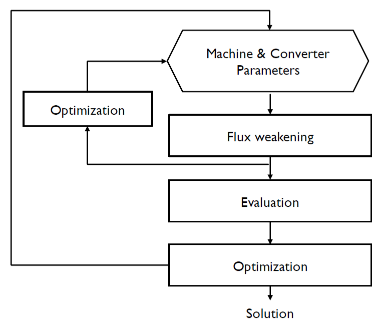
\includegraphics[width=0.5\textwidth]{loop.png}
    \caption{Optimisation imbriquée}
\end{figure}
On a toute une série d'équation qui forment le modèle analytique :
\begin{itemize}
    \item Modèle électrique de la machine en fonction du paramètre nombre de paires de pôles.
    \item Modèle des pertes cuivre et fer en fonction des paramètres géométriques (résistance au stator), le nombre de paires de pôles et le maximum local du champ magnétique (dépend des paramètres géométriques).
    \item Modèle magnétique en fonction des paramètres géométriques, du nombre de tours des bobinages et du nombre de paires de pôles.
    \item Modèle des pertes dans les IGBT.
    \item Modèle du couple selon les vagues.
\end{itemize}
Avec toutes ces équations, on peut faire une optimisation avec stratégie PSO.

\subsubsection{Évaluation et interprétation des résultats}
Est-ce que c'était pertinent de s'inquiéter du défluxage (i.e courant $i_d$) ? Oui. Le front de Pareto nous montre bien qu'une machine correctement défluxée peut atteindre une puissance électrique plus grande avec un coût plus faible. L'ingénieur n'a plus qu'à choisir la machine dont il a besoin selon les objectifs coût/énergie électrique.
\begin{figure}[H]
    \centering
    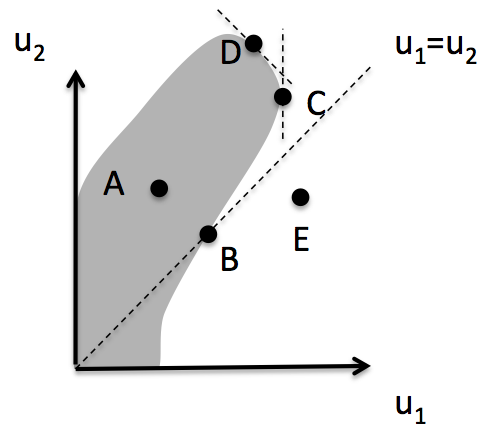
\includegraphics[width=0.65\textwidth]{pareto.png}
    \caption{2 fronts de Pareto : machine défluxée et machine non-défluxée.}
\end{figure}
